This section explains the results of the project in \ref{subsec:results} and evaluate on the results in \ref{subsec:evaluation}.

\subsection{Results}
\label{subsec:results}
The Results section contains results for both the preprocessing and the two classification algorithms and their performance.


\subsubsection{Preprocessing}
The preprocessing was done in the following setting.
Initially the images was downscaled to 100 pixels width.
Images was normalized using Z-Score normalization resulting in the right image of Figure \ref{fig:step1}. By normalizing the images the contrasts in the becomes greater and this will ease the separation.
In the next step, the image is smoothed with a Gaussian smoothing algorithm with a sigma level of 2. This equalizes the values of the individual pixels a bit and there by make neighboring pixel more alike.
When these steps are done, two features are extracted from each pixel.
These features are the redness and a gray scale value.
The features are then used for the kMeans clustering algorithm.
The clusters are constructed using Euclidean distances. Further is the algorithm constructed to build 4 different clusters.
The reason for using four clusters, is that it is expected that water will be grouped into one, water splashes into another and whale into one and lastly one cluster for "garbage". 

When the clusters are created the next step  is to identify which cluster(s) the whale have been added to.
This is done by finding the cluster which has the highest rate of redness within. This works for most of the images but not all. In some images the contrast between whale and water is not high enough or the light when the image was taken makes the water splashes red. When this happens, the cluster correct cluster is chosen by calculating the center of gravity in the image. After the center of gravity is calculated the cluster in which it is placed is picked, if the size of that cluster is between 5 \% and 20 \% of the total. This is picks out the correct cluster with a accuracy of around 50 \%.
When it fail to find a cluster, a cluster matching the size for 10-15 \% of the total image is taken \footnote{Note that the last approach might chose a wrong cluster, and cannot be validated, which is why the two other approaches are preferred}. 

When one or more cluster is chosen, everything not in that cluster is filtered out from the original smoothed image as seen in Figure \ref{fig:step3} right. The whole process is then repeated once more in order to filter out some few water pixels which was gathered in the whale cluster.
After the second round a minimum bounding box is calculated around the whale cluster, and the image is then cropped.

\begin{figure}
\centering
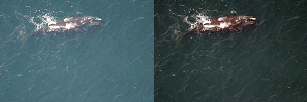
\includegraphics{Images/preprocess1}
\end{figure}

\subsubsection{Random Forest}
The Results for Random Forest is split into two sections. As there has been conducted classification for both data which was just resized and data which has been additionally preprocessed before resizing.

\paragraph{The Resized Data} 
Contains the results which is shown in \ref{fig:??}. As 


\subsubsection{Neural Network}



\subsection{Evaluation}
\label{subsec:evaluation}